\documentclass[slovene,11pt,a4paper]{article}
\usepackage[margin=1.8cm,bottom=3cm,foot=1.5cm]{geometry}
\usepackage{amsmath}
\usepackage{booktabs}
\usepackage{float}
\usepackage{graphicx}
\usepackage{gensymb}
\usepackage{geometry}
\usepackage{changepage}
\usepackage{subcaption}
\usepackage{multirow}
\usepackage{blindtext}
\usepackage{hyperref}
\usepackage[version=4]{mhchem}
\usepackage[slovene]{babel}
\pagenumbering{gobble}
\renewcommand{\contentsname}{\centering Contents}

\begin{document}

\title{10. naloga - Spektralna analiza in filtriranje}
\author{Tadej Lozej 28201055}
\maketitle
\begin{center}
Modelska analiza 1 \\
\bigskip
Predavatelj: prof. dr. Simon Širca \\
Asistent: doc. dr. Miha Mihovilovič
\end{center}

\newpage

\tableofcontents

\newpage

\section{Uvod}

\pagenumbering{arabic}

V nalogi se bomo posvetili spektralni analizi in filtriranju. Uporabljali bomo diskretno Fourierovo transformacijo ter Wienerjev filter. Uporabljene signale dobimo na spletni strani predmeta Modelska analiza 1.

\section{Frekvenčni spekter}

Signaloma s 512 točkami na datotekah \texttt{val2.dat} in \texttt{val3.dat} želimo določiti frekvenčni spekter. Na sliki 1 sta prikazana ta dva signala v odvisnosti od časa.

\begin{figure}[h!]
\centering
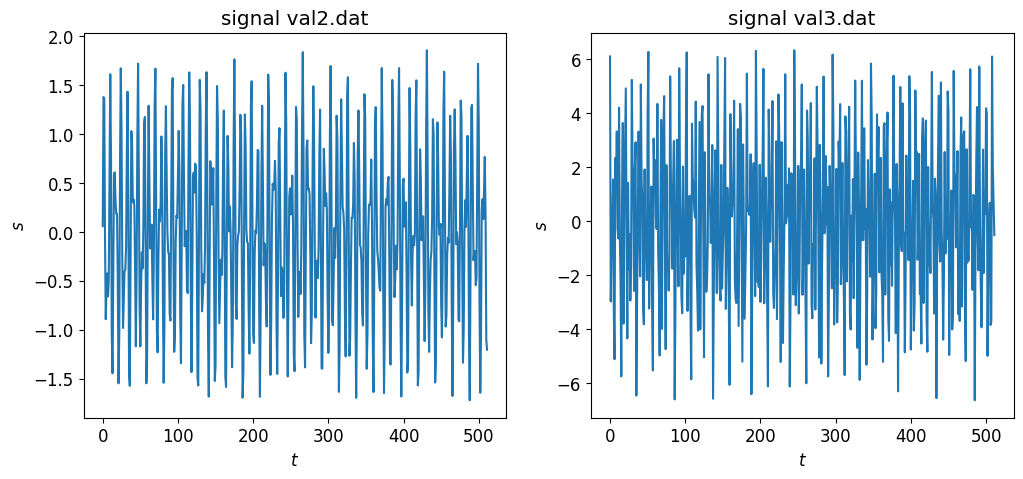
\includegraphics[width=12cm]{slika1.png}
\caption{Signala na datotekah \texttt{val2.dat} in \texttt{val3.dat} v odvisnosti od časa.}
\end{figure}

Frekvenčni spekter teh dveh signalov bomo dobili s pomočjo diskretne Fourierove transformacije. Slednja deluje tako, da za izračun $k$-te komponente Fourierove transformiranke signala $S_k$ moramo pomnožiti vse točke v signalu $s_k$ z uztreznim eksponentnim faktorjem

\begin{equation}
S_k = \sum_{j=0}^{N-1} w_j s_j e^{-i 2\pi jk/N},
\end{equation}
kjer je $w_j$ ustrezna komponenta okenske funkcije ter $N$ število točk v signalu. Raziskali bomo več okenskih funkcij in sicer:

\begin{itemize}
\item Brez okna \[ w_j = 1, \]
\item Bartlett \[ w_j = 1 - \frac{|j- N/2|}{N/2}, \]
\item Hann \[ w_j = \frac{1}{2} \left( 1-\cos \frac{2\pi j}{N} \right), \]
\item Welch \[ w_j = 1 - \left( \frac{j - N/2}{N/2} \right)^2, \]
\item Gauss \[ w_j =  e^{-\left( \frac{j - N/2}{\sigma} \right)^2}, \] kjer je $\sigma$ parameter za katerega si izberemo vrednost $\sigma = 100$.
\end{itemize}
Na sliki 2 so prikazane uporabljene okenske funkcije.

\newpage

\begin{figure}[h!]
\centering
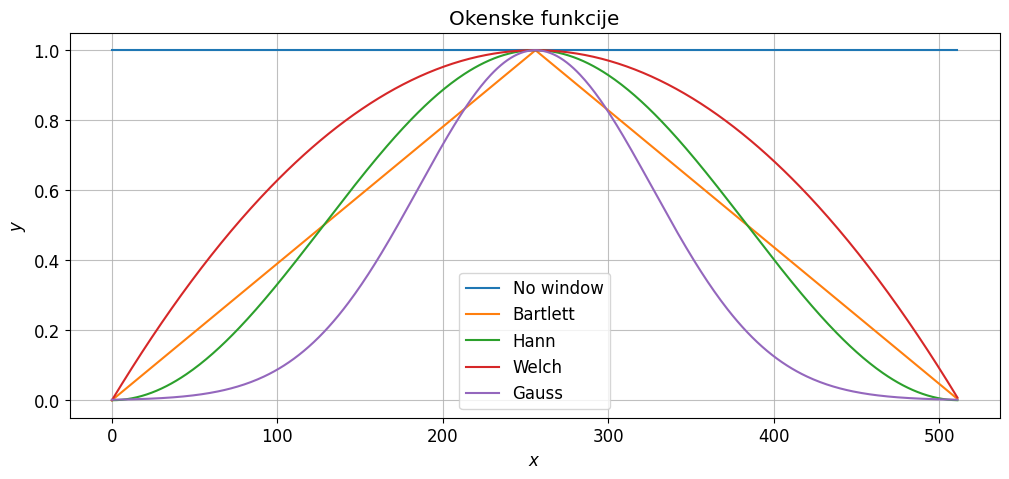
\includegraphics[width=12cm]{slika2.png}
\caption{Uporabljene okenske funkcije pri diskretni Fourierovi transformaciji.}
\end{figure}

Iz Fourierove transformiranke signala nato dobimo spekter oz. spektralno gostoto kot

\begin{equation}
2P_k = \frac{1}{W}(|S_k|^2 + |S_{N-k}|^2); \quad k \in (0, N/2),
\end{equation}
kjer je $W = \sum_j w_j^2$. Spektralna gostota ima le $N/2$ točk in jo opazijemo v frekvenčnem prostoru. Teh $N/2$ točk je enakomerno porazdeljeno po intervalu $(0, \nu_c)$, kjer je $\nu_c = \frac{1}{2\Delta t}$ kritična frekvenca, ki je odvisna od pogostosti vzorčenja signala $\Delta t$. V našem primeru je $\Delta t = 1$ ter kritična frekvenca tako znaša $\nu_c = 0.5$. Bolj fino kot signal vzorčimo višje frekvence smo sposobni zaznati. Na sliki 3 sta v logaritemski skali prikazani spektralni gostoti signalov iz datotek \texttt{val2.dat} ter \texttt{val3.dat}. V spektralni gostoti signala \texttt{val2.dat} opazimo dva očitna vrhova, ki sta pobližje prikazana na manjših grafih. Vrhova se nahajata za vsa okna pri frekvencah $\nu_1^{(1)} = 0,133$ ter $\nu_2^{(1)} = 0,220$. Pri prvem spektru na prvi pogled ne vidimo prav velikih razlik med tem ali okno uporabimo ali ne. Veliko očitnejša razlika je pri drugem spektru. Tukaj opazimo štiri vrhove in prav vsi so v logaritemski skali bolj očitni če uporabimo katerokoli

\begin{figure}[h!]
\centering
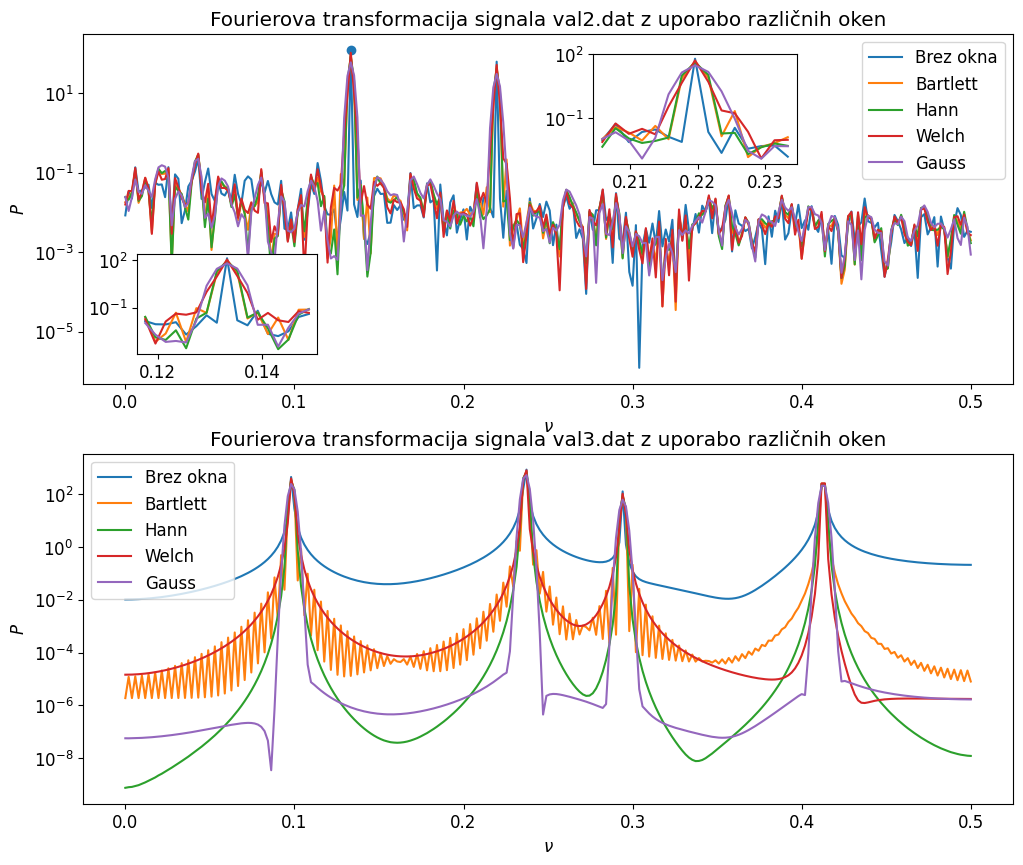
\includegraphics[width=12cm]{slika3.png}
\caption{Spektralni gostoti signalov iz datotek \texttt{val2.dat} (zgoraj) ter \texttt{val3.dat} (spodaj).}
\end{figure}

\newpage

\noindent okensko funkcijo. Na prvi pogled z Gaussovo okensko funkcijo dosežemo najboljše rezultate. Prvi trije vrhovi na drugem grafu se v vseh spektrih nahajajo na istih frekvencah, in sicer $\nu_1^{(2)} = 0,098$, $\nu_2^{(2)} = 0,238$ ter $\nu_3^{(2)} = 0,294$. Položaj zadnjega vrha pa se za različna okna razlikuje na tretji decimalki. Spektralna gostota brez okna in Gauss postavita četrti vrh na $\nu_4^{(2)} = 0,0414$, ostale tri metode pa na frekvenco $\nu_4^{(2)} = 0,412$. Gre za precej majhno razliko, ki verjetno pride v igro zaradi premajhnega števila točk v signalu.

Pobližje si poglejmo lastnosti dveh vrhov v spektralni gostoti prvega signala (signal iz datoteke \texttt{val2.dat}). Na sliki 4 in 5 so prikazani histogrami, ki prikazujejo višino vrhov, FWHM vrhov, prominence vrhov ter prominence vrhov logaritmiranega spektra. Prominence je lastnost vrhova, ki meri koliko vrh odstopa od signala okrog njega. Definirana je kot razdalja med vrhom in njegovo konturo. Pominence vrhov logaritmiranega spektra (desetiški logaritem) nam da upogled v to za koliko velikostnih redov se vrh razlikuje od njegove konture. To se mi zdi precej dober kvalifikator za določitev uspešnosti različnih oken, saj vrh v logaritemski skali spektra lažje zaznamo, če se od svoje konture razlikuje za več velikostnih redov.

\begin{figure}[h!]
\centering
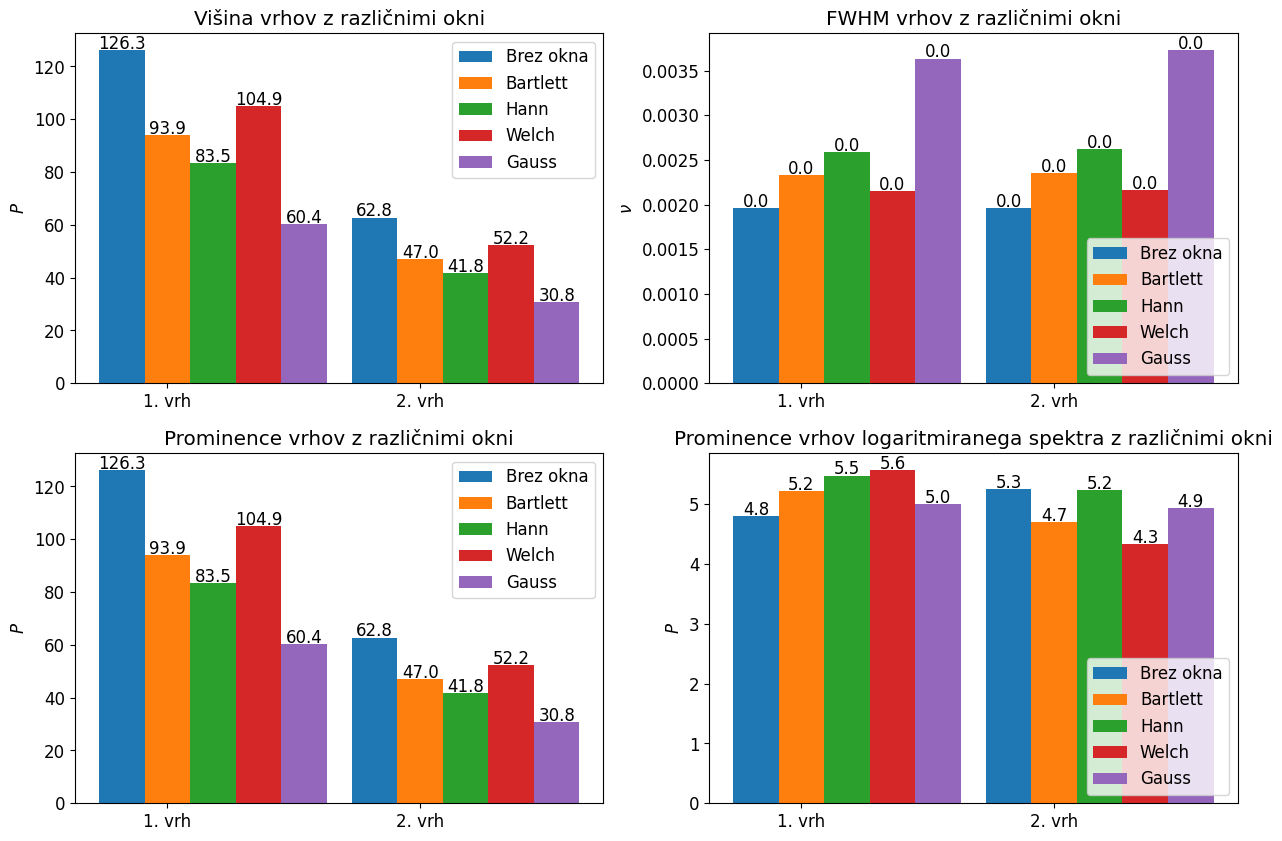
\includegraphics[width=15cm]{slika4.png}
\caption{Stolpični diagrami, ki prikazujejo različne lastnosti dveh vrhov v spektralni gostoti signalov iz datoteke \texttt{val2.dat}.}
\end{figure}

Najvišje ter najožje vrhove nam vrne sama Fourierova transformacija brez okna. Po vrsti v širini ter višini nato sledijo okna Welch, Bartlett, Hann in Gauss. Prominence vrhov spektra je na prvi decimalki enak kot njihova višina, saj je kontura vrhov precej majhna. Vidimo pa, da pri prominence vrhov logaritmiranega spektra nastopijo vsa okna precej podobno. Oba vrhova se pri uporabi kateregakoli okna od svoje konture ločita za približno pet velikostnih redov. Te ugotovitve se zdijo smiselne, saj če pogledamo zgornji graf na sliki 3 tudi na prvi pogled zgleda kot da to drži. Nemoremo pa enako trditi za  spodnji graf na sliki 3.

Podobno analizo vrhov lahko storimo tudi za štiri vrhove v spektralni gostiti signala iz datoteke \texttt{val3.dat}. To je prikazano na sliki 5. Vidimo, da nam Fourierova transformacija brez okna vrne prve tri vrhove najvišje in najožje. Nato za te tri kot prej sledijo Welch, Bartlett, Hann in Gauss. Če pogledamo četrti stolpični diagram pa vidimo jasne razlike med uporabljenimi okenskimi funkcijami. V logaritemski skali najbolj iztopajo vrhovi spektralne gostote, ki jih dobimo z uporabo okenske funkcije Hann in Gauss, kar lahko s pogledom na spodnji graf slike 3 potrdimo, Sledijo Bartlett, Welch ter šele nato metoda brez okna.

\begin{figure}[h!]
\centering
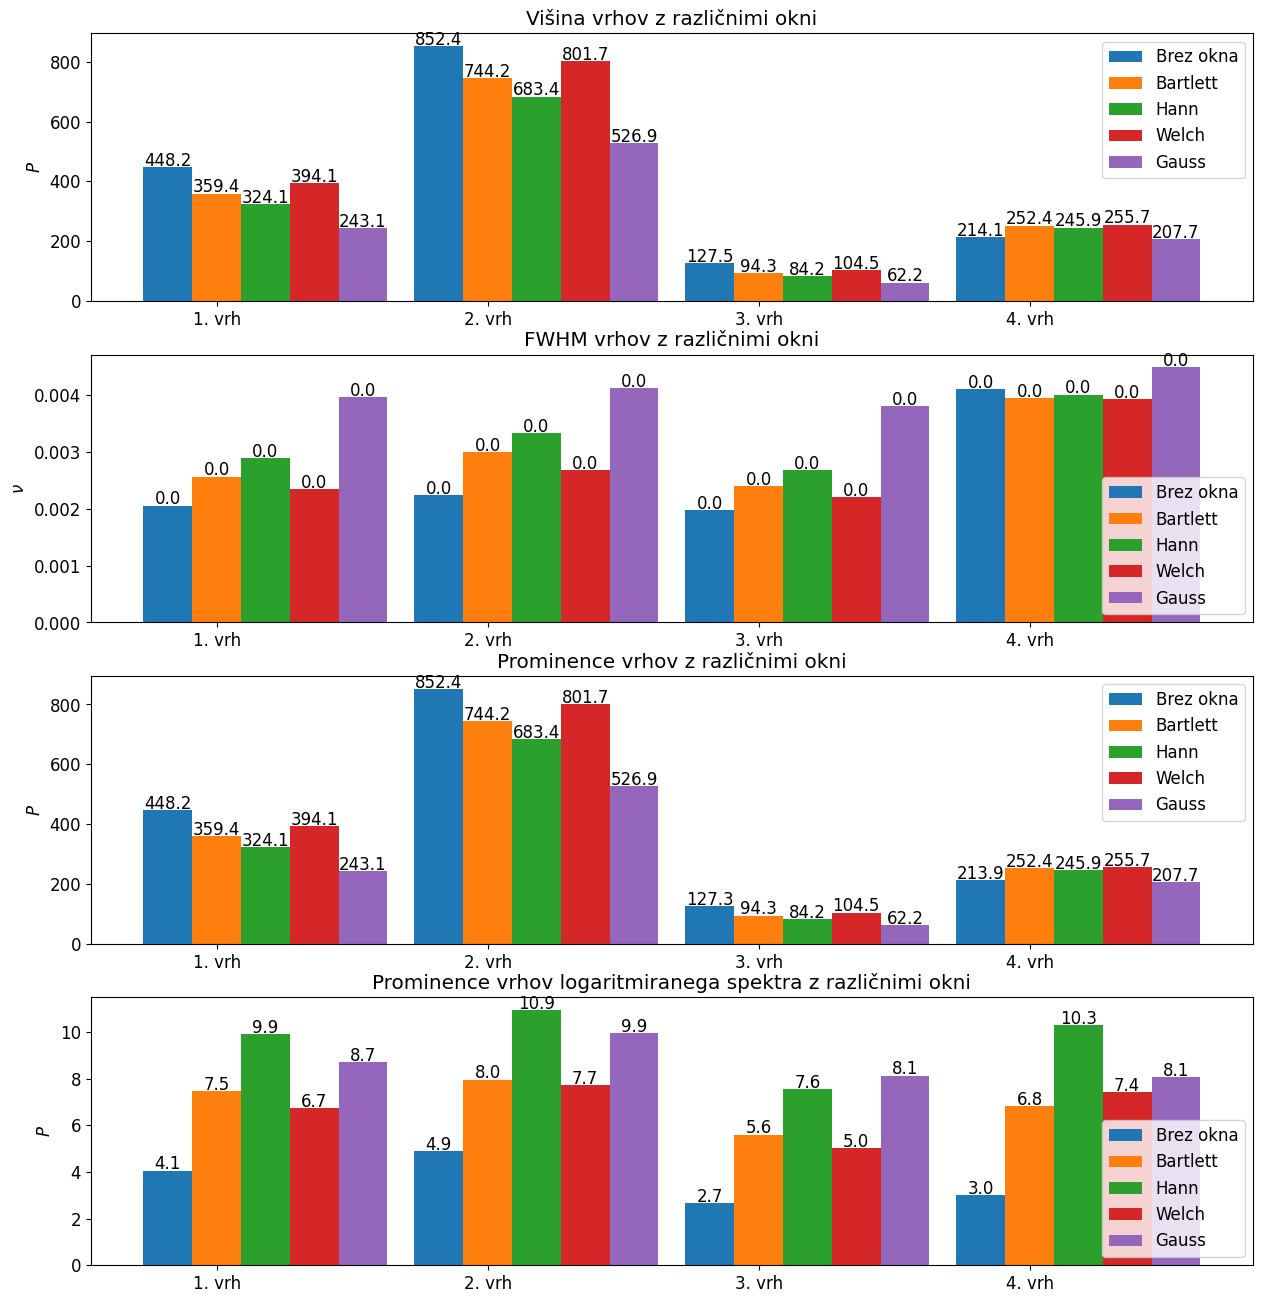
\includegraphics[width=15cm]{slika5.png}
\caption{Stolpični diagrami, ki prikazujejo različne lastnosti dveh vrhov v spektralni gostoti signalov iz datoteke \texttt{val3.dat}.}
\end{figure}

\subsection{Manj točk signala}

Poglejmo si, kaj se zgodi s spektralno gostoto signala, če za signal vzamemo le prvih 256 točk in ne vseh 512. To nam razpolovi število frekvenčnih točk na intervalu $(0, \nu_c)$. Na sliki 6 je prikazan rezultat. Vidimo, da so vrhovi v tem primeru predvsem širši. Če bolj podrobno pogledamo lahko opazimo, da je tudi prominence teh vrhov manjši. Dobro pa je to, da še vedno razločimo v zgornjem spektru dva vrhova ter v spodnjem štiri.

Na sliki 7 so prikazani stolpični diagrami nekaj lastnosti vrhov za različna uporabljena okna enako kot v poglvju 1. Vidimo, da za razliko od prej, sedaj Gauss vrne višje in ožje vrhove kot ostala uporabljena okna. Razlike v velikostnih redih med vrhom in njegovo konturo so rahlo manjše kot če uporabimo vseh 512 točk. Vrhovi so nižji in prav tako je FWHM vseh vrhov približno 10 krat večji.

Enaka analiza je prikazana še na sliki 8 za signal iz datoteke \texttt{val3.dat}. Spet vidimo, da je Gauss vrnil druge najbolj visoke ter ozke vrhove za razliko od prej. So pa vsi vrhovi približno enkrat nižji od prejšnjih. Prav tako so približno enkrat širši kot prej in vrhovi se z njihovimi konturami razlikujejo za manj velikostnih redov.

\begin{figure}[h!]
\centering
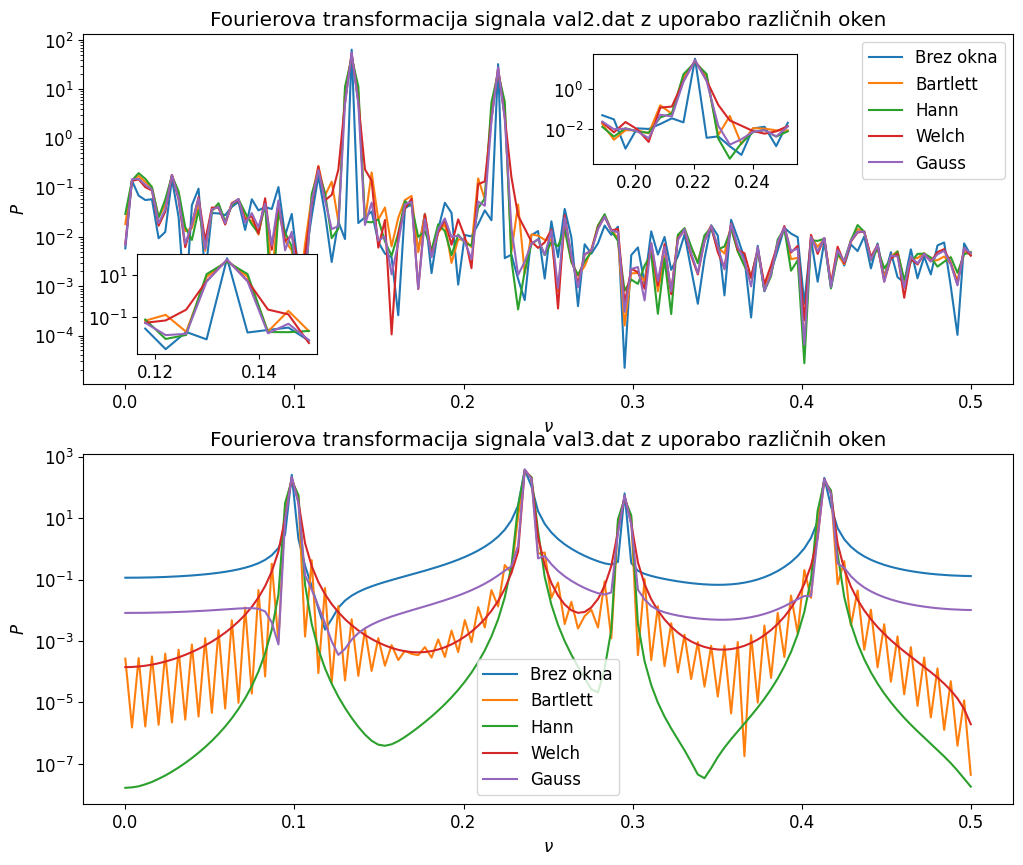
\includegraphics[width=12cm]{slika6.png}
\caption{Spektralni gostoti signalov iz datotek \texttt{val2.dat} (zgoraj) ter \texttt{val3.dat} (spodaj), če vzamemo le prvih 256 točk signala.}
\end{figure}

\begin{figure}[h!]
\centering
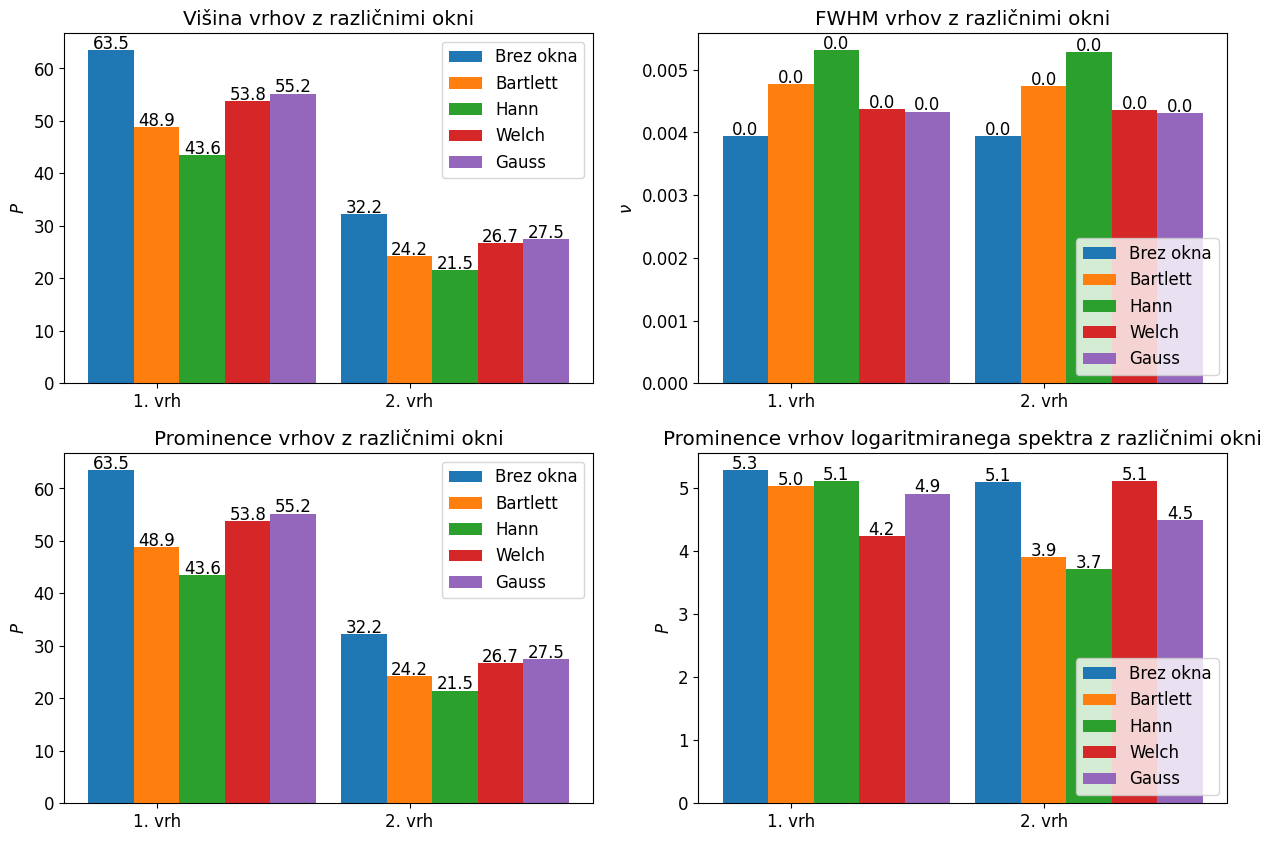
\includegraphics[width=15cm]{slika7.png}
\caption{Stolpični diagrami, ki prikazujejo različne lastnosti dveh vrhov v spektralni gostoti signalov iz datoteke \texttt{val2.dat}, če vzamemo le prvih 256 točk signala.}
\end{figure}

\newpage

\begin{figure}[h!]
\centering
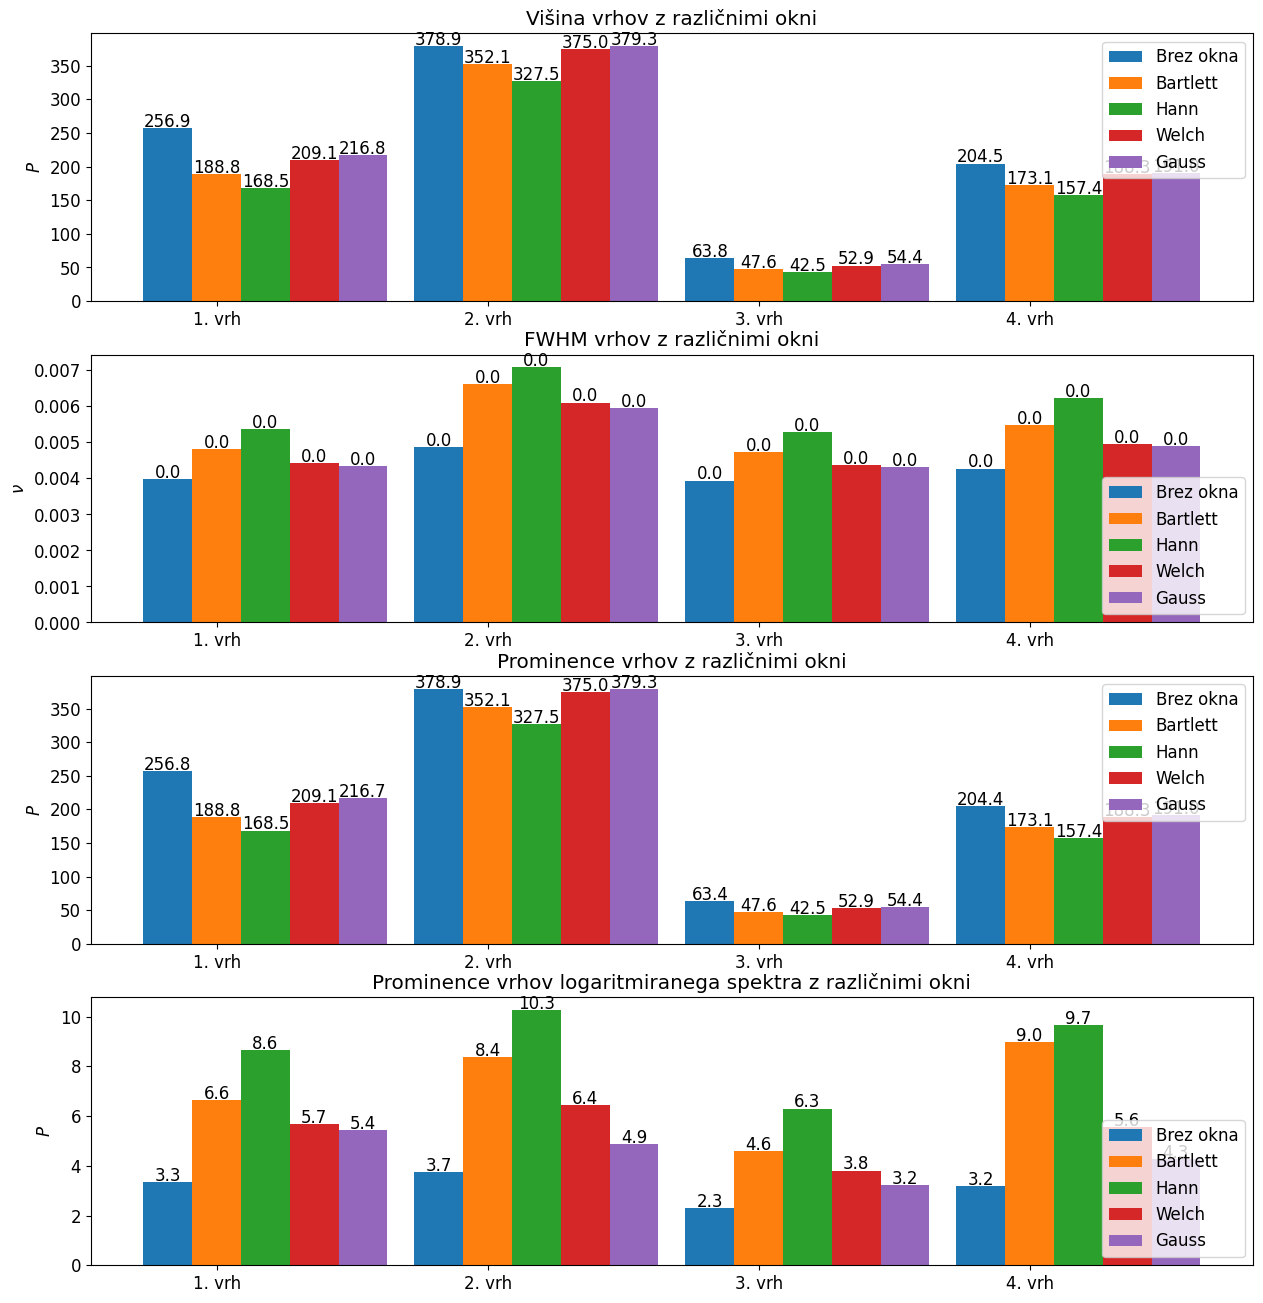
\includegraphics[width=15cm]{slika8.png}
\caption{Stolpični diagrami, ki prikazujejo različne lastnosti dveh vrhov v spektralni gostoti signalov iz datoteke \texttt{val3.dat}, če vzamemo le prvih 256 točk signala.}
\end{figure}

Pričakujemo lahko, da manj točk kot vzamemo nižji ter bolj široki bojo vrhovi oz. zmeraj težje bomo opazili vrhove, saj bomo zmeraj bolj redčili število frekvenc na intervalu. Na sliki 9 si poglejmo kako so tri lastnosti vrhov v spektralni gostoti odvisne od tega koliko točk signala \texttt{val2.dat} vzamemo. Vidimo nihajoče obnašanje vseh lastnosti. To je posledica puščanja, saj želimo s točkami zadeti točno periodo signala za najboljše rezultate. V splošnem pa vidimo naraščajoč trend pri višini ter prominence-i vrhov ter padajoč trend pri širini vrhov. Če pozorno pogledamo vidimo, da Gauss po nekem številu zajetih točk začne stagnirati. Na začetku vrača Gauss precej visoke in najbolj ozke vrhove a ga kasneje druge okenske funkcije premagajo. To zna biti posledica slabo izbranega parametra $\sigma$.

\newpage

\begin{figure}[h!]
\centering
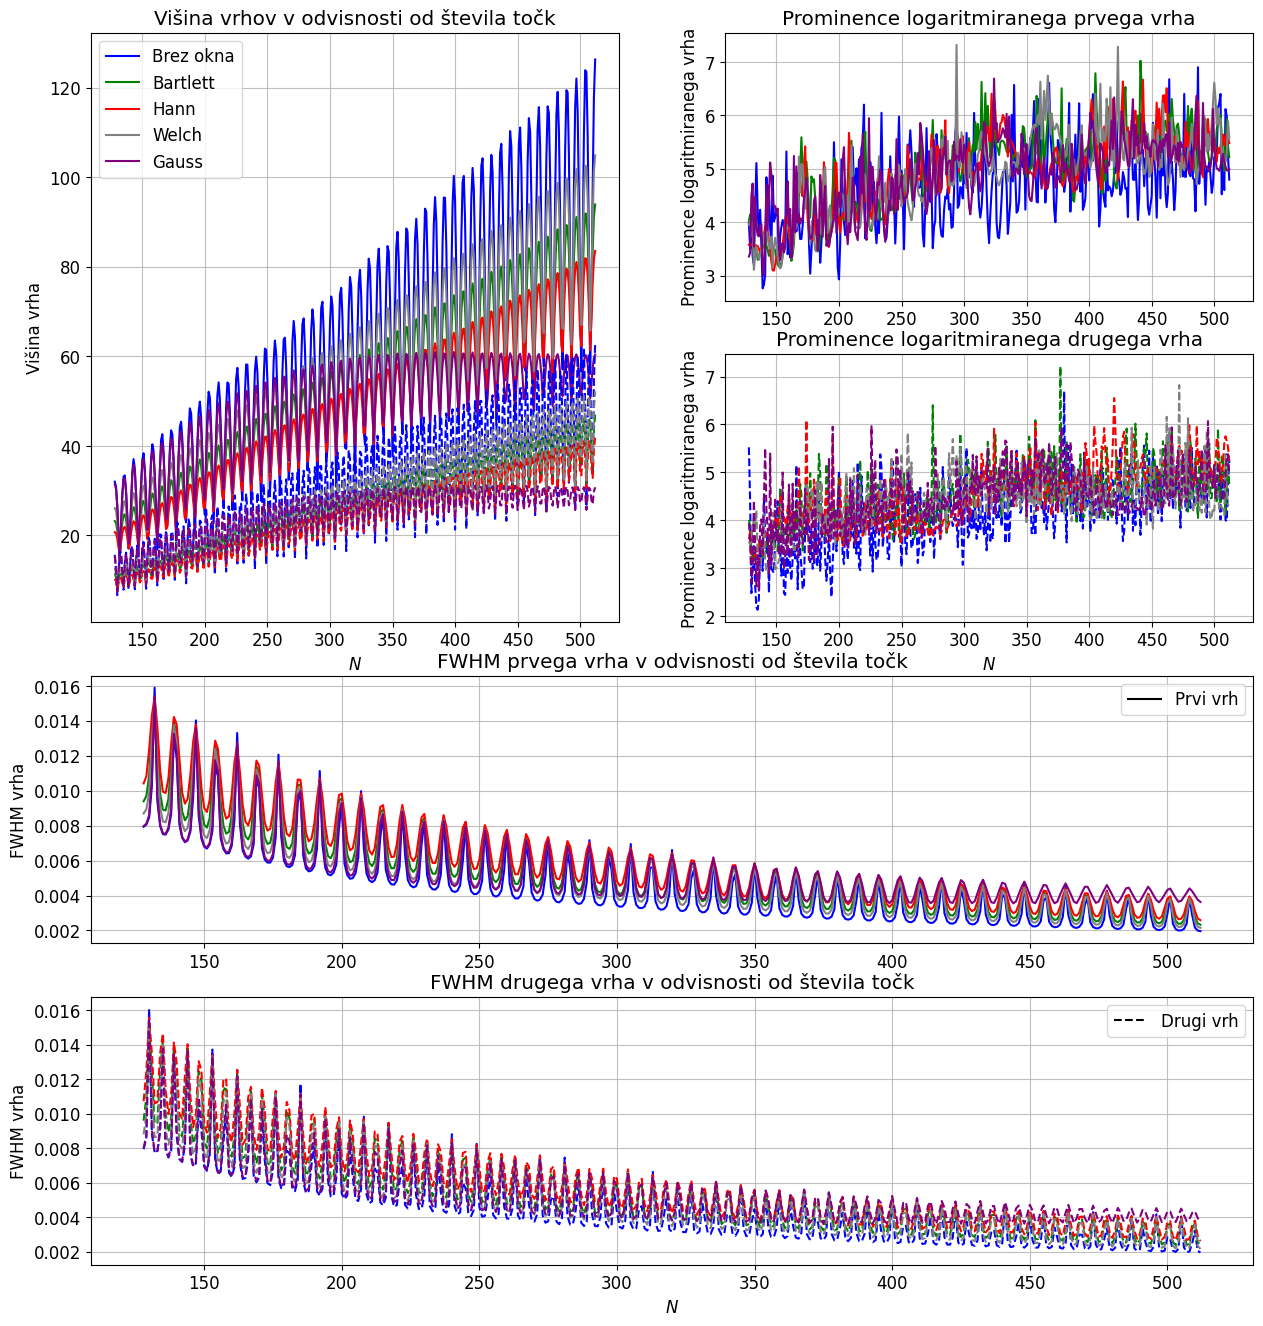
\includegraphics[width=15cm]{slika9.png}
\caption{Slika prikazuje višini, prominence-i logaritmiranih ter FWHM-ja prvega ter drugega vrha spektralne gostote signala iz datoteke \texttt{val2.dat} v odvisnosti od tega koliko točk iz siglana vzamemo.}
\end{figure}

Na sliki 10 vidimo enako analizo za vse štiri vrhove spektralne gostote signala iz datoteke \texttt{val3.dat}. Tukaj vidimo precej bolj očitno razliko med različnimi okenskimi funkcijami kot v prejšnjem primeru. Trendi so seveda pričakovano enaki in prav tako opazimo nihajočo naravo vseh lastnosti zaradi pojava puščanja. Vidimo, da najvišje vrhove konstantno dobijamo brez uporabe okna, vendar vrhove v logaritemski skali najlažje ločimo, če uporabimo okensko funkcijo Hann. V tem primeru vse šriti vrhove lahko ločimo od svojih kontur tudi za 10 velikostnih redov.

\newpage

\begin{figure}[h!]
\centering
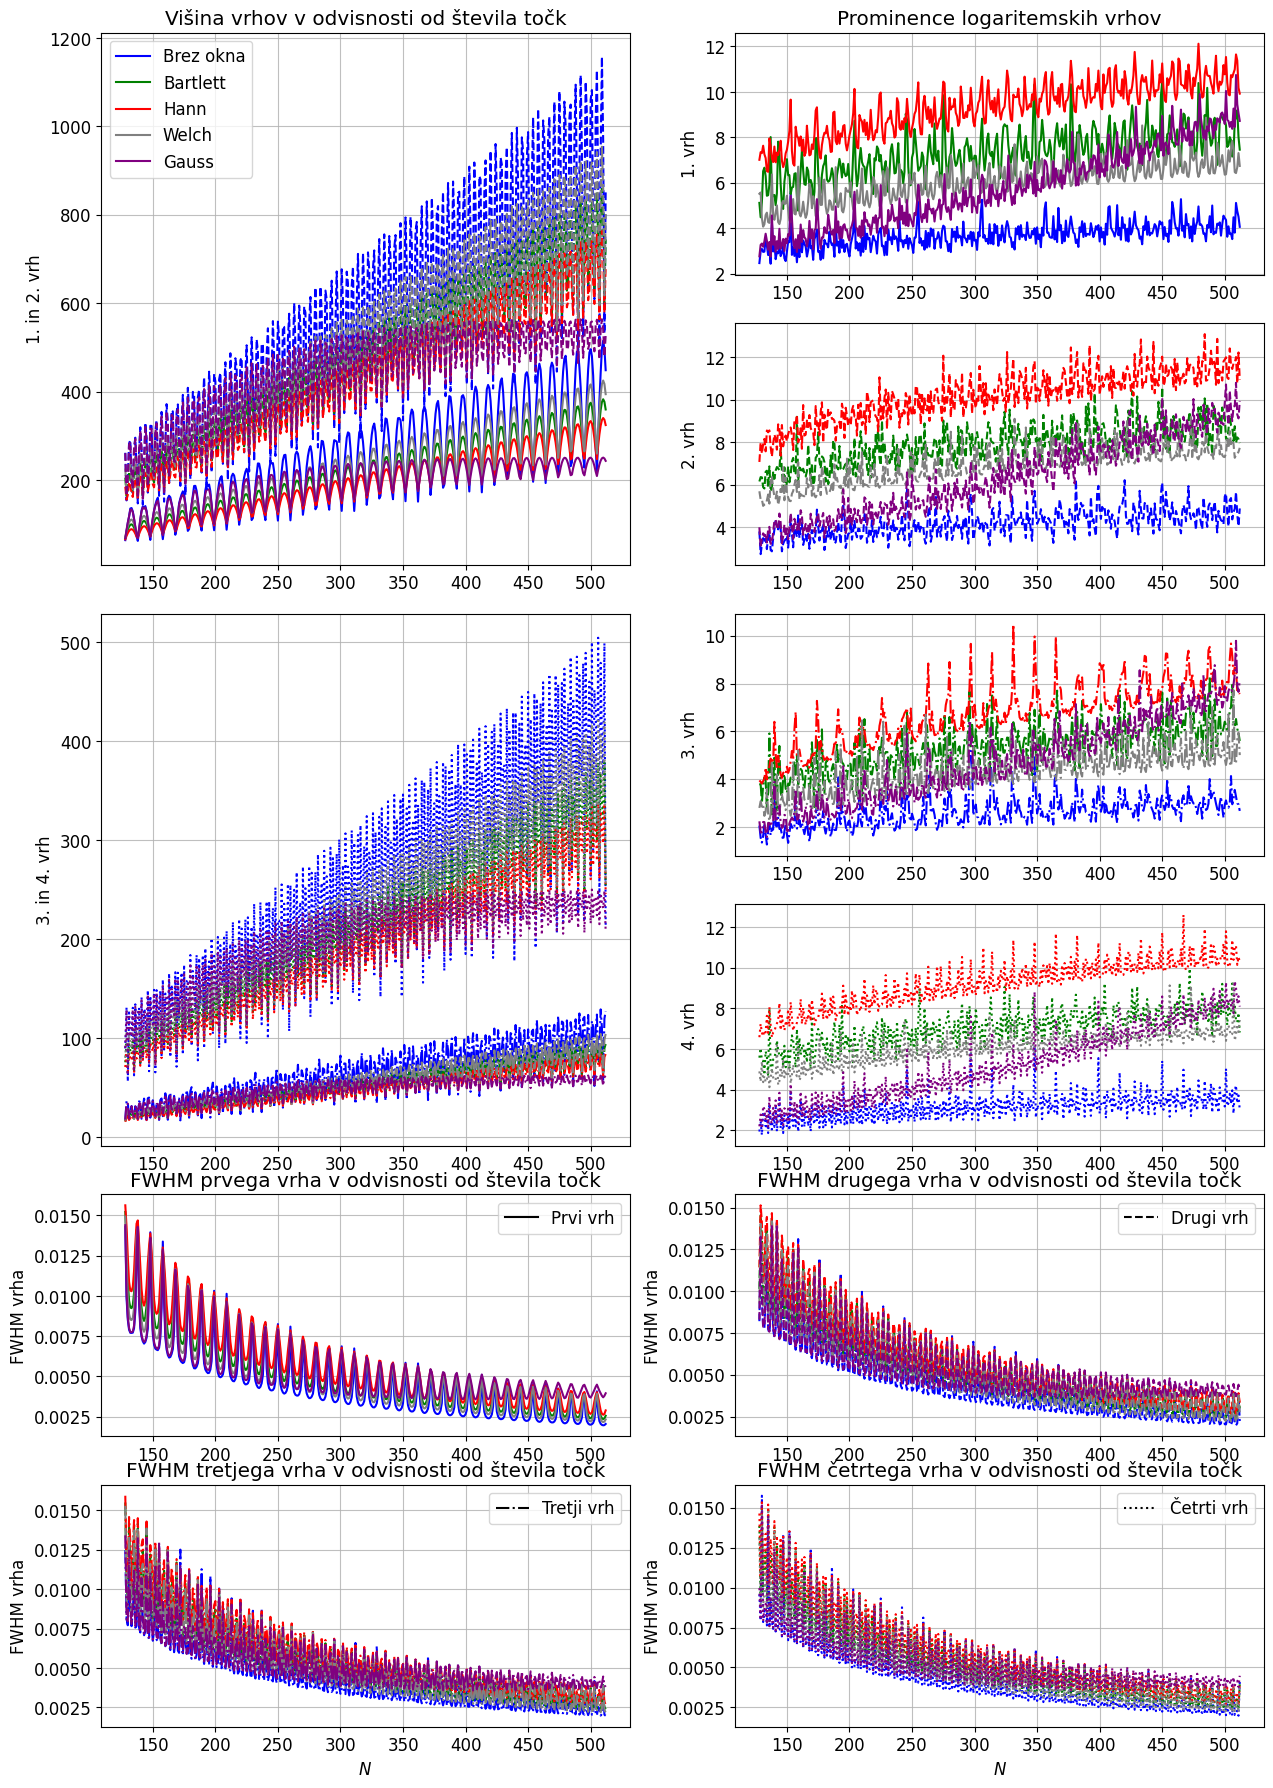
\includegraphics[width=15cm]{slika10.png}
\caption{Slika prikazuje višine, prominence logaritmiranih ter FWHM-je prvega, drugega, tretjega ter četrtega vrha spektralne gostote signala iz datoteke \texttt{val3.dat} v odvisnosti od tega koliko točk iz siglana vzamemo.}
\end{figure}

\newpage

\section{Wienerjev filter}

Signal $u(t)$, ki prihaja v merilno napravo s prenosno funkcijo $r(t)$, se ob dodatku šuma $n(t)$ preoblikuje v 

\begin{equation}
c(t) = u(t) * r(t) + n(t) = s(t) + n(t).
\end{equation}
Iz izmerjenega časovnega poteka $c(t)$ bi radi, ob poznavanju odzivne funkcije $r(t)$ in ob nekaterih predpostavkah o šumu $n(t)$, rekonstruirati vpadni signal $u(t)$. N. Wiener je predlagal naslednjo rešitev, ki sledi iz minimizacije napake po metodi najmanjših kvadratov. Pred dekonvolucijo je treba transformiranko $C(f)$ pomnožiti s filtrom 

\begin{equation}
\Phi (f) = \frac{|S(f)|^2}{|S(f)|^2+|N(f)|^2}.
\end{equation}

Naloga je s pomočjo Wienerjevega filtra napraviti dekoncolucijo signalopv iz datotek na spletni strani predmeta modelska analiza 1 \texttt{signal\{0,1,2,3\}.dat}. Signali so prikazani na sliki 11.

\begin{figure}[h!]
\centering
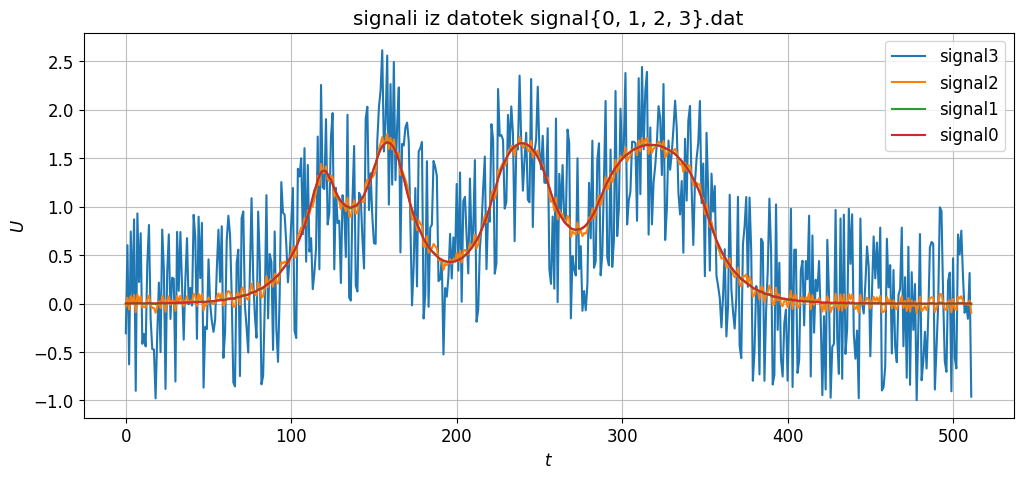
\includegraphics[width=12cm]{slika11.png}
\caption{Signali iz datotek \texttt{signal\{0,1,2,3\}.dat}. Prvi ni zašumljen, naslednji so pa postopoma vedno bolj.}
\end{figure}

Signal iz datoteke \texttt{signal0.dat} ni zašumljen in dekonvolucijo lahko opravimo brez filtra. Opravimo jo na sledeč način.

\begin{equation}
u = F_N^{-1} \left[ \frac{C(f)}{R(f)} \right],
\end{equation}
kjer je $C(f)$ Fourierova transformiranka merjenega signala ter $R(f)$ Fourierova transformiranka prenosne funkcije merilne naprave. Na sliki 12 vidimo, da je originalen signal, ki smo ga merili škatlast. Tak pristop je pri zašumljenih signalih neuporaben.

Na sliki 13 so prikazani rezultati dobljeni s uporabo Wienerjevega filtra. Vidimo, da pri vseh signalih lahko bolje rekonstruiramo resnični škatlast signal. Za vrednost šuma sem vzel povprečje vrednosti po rdeči piki na vsakem grafu za vrednost signala sem pa ročno prilagajal ensponentno funkcijo (na log skali premico) podatkom pred rdečo piko.

\newpage

\begin{figure}[h!]
\centering
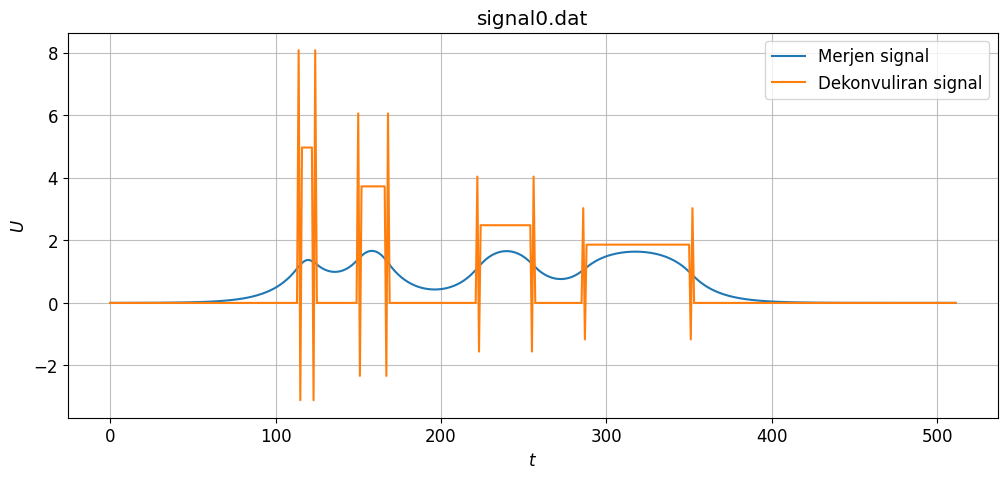
\includegraphics[width=12cm]{slika12.png}
\caption{Signal $c_0 $ iz datoteke \texttt{signal0.dat} in dekonvuliran signal $s_0$.}
\end{figure}

\begin{figure}[h!]
\centering
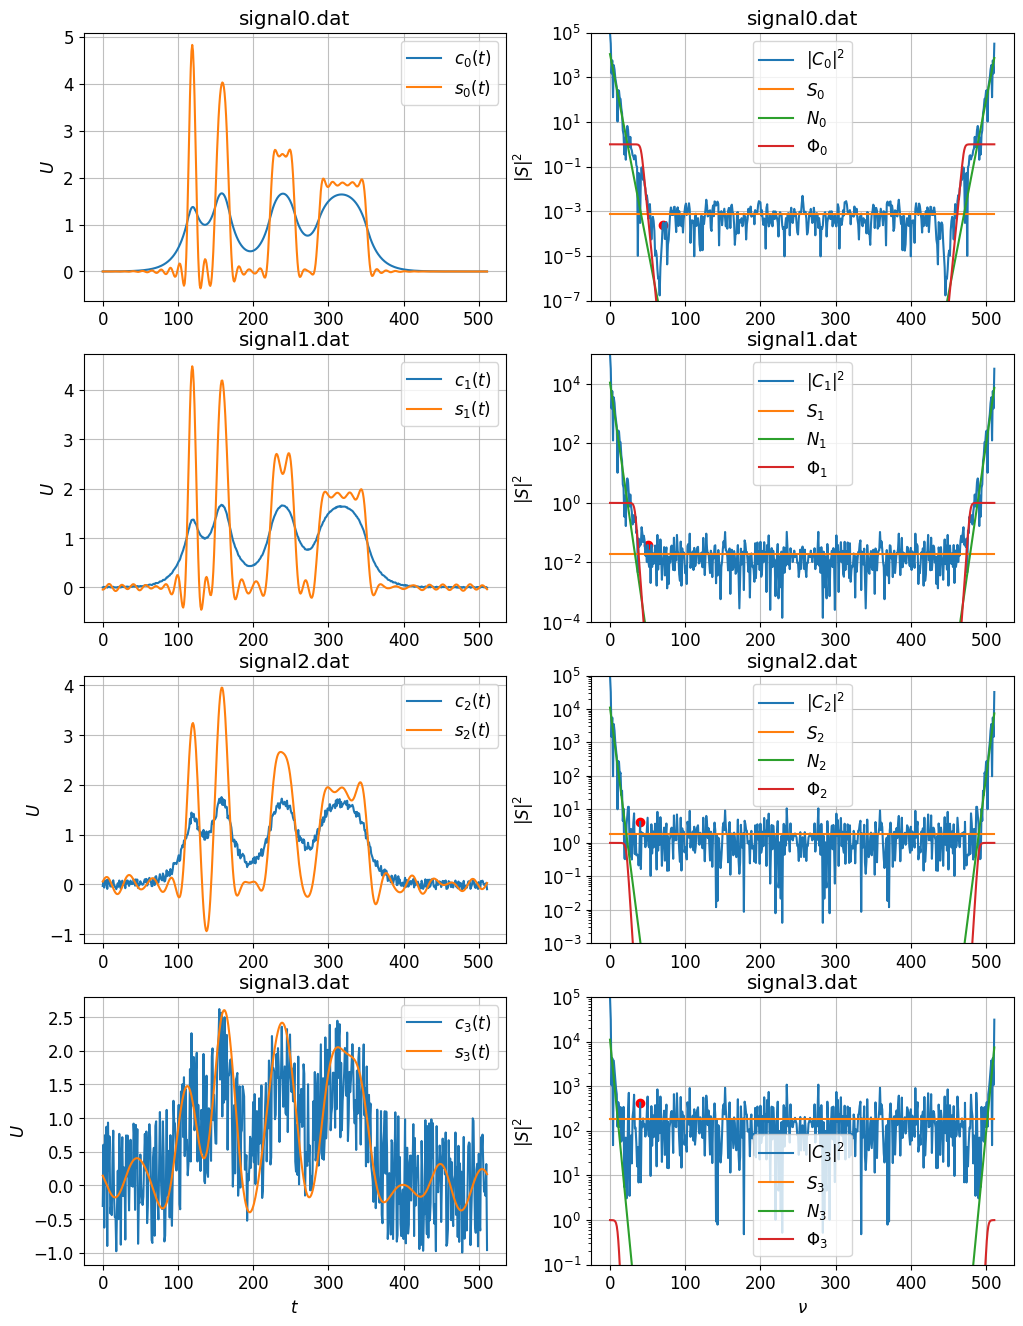
\includegraphics[width=12cm]{slika13.png}
\caption{Signal $c_0 $ iz datoteke \texttt{signal0.dat} in dekonvuliran signal $s_0$.}
\end{figure}

\newpage

\section{Lena}

V fotografiji imamo pogosto opravka s popačitvami konvolucijske narave: razmazanje zaradi gibanja, tresenje objektiva med ekspozicijo, slabo fokusiranje, različne optične aberacije. V primeru, da poznamo prenosno funkcijo, lahko posežemo po dekonvolucijskih metodah, s katerimi lahko do neke mere rekonstruiramo originalno fotografijo, odvisno seveda od zrnatosti fotografije.

Poskusili bomo očistiti podobe Lene (\texttt{lena\_k\{1,2,3\}\_n\{0,4,8,16\}.pgm}) v arhivu na spletni učilnici predmeta modelska analiza 1. Imamo tri znana konvolucijska jedra, ki predstavljajo tresoč objektiv (\texttt{kernel1.pgm}), slab fokus (\texttt{kernel2.pgm} ter uklonska mrežica (\texttt{kernel3.pgm}). Konvolucijska jedra so prikazana na sliki 14. Datotekam je primešana različna količina Gaussovskega šuma ($\text{RMS} = 0, 4, 8, 16$).

\begin{figure}[h!]
\centering
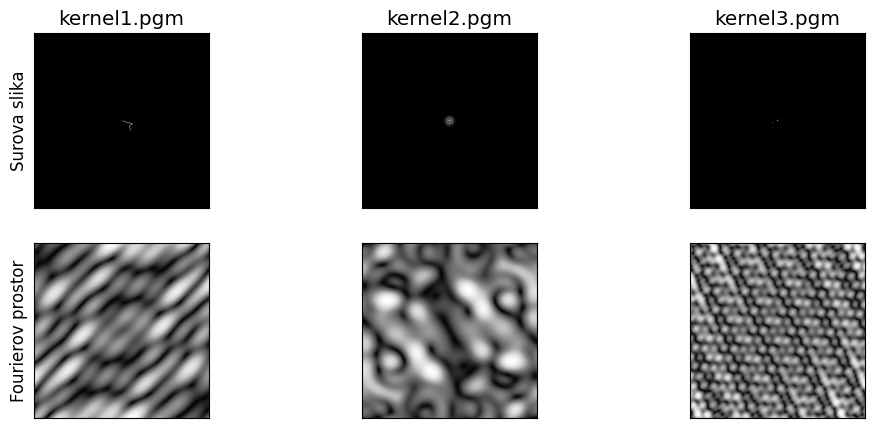
\includegraphics[width=12cm]{slika14.png}
\caption{Različna konvolucijska jedra v datotekah \texttt{kernel1.pgm}, \texttt{kernel2.pgm} in \texttt{kernel3.pgm}, ki po vrsti predstavljajo tresoč objektiv, slab fokus ter uklonsko mrežico.}
\end{figure}

Pri filtriranju smo uporabili Wienerjev filter

\begin{equation}
\Phi(u, v) = \frac{|S|^2}{|S|^2 + C},
\end{equation}
kjer je $S$ naš merjeni signal signal ter $C$ nek konstanten šum, ki sem ga ročno spreminjal tako, da sem dobil na videz najboljši rezultat. Za takšno konstrukcijo filtra sem se odločil, ker nisem točno vedel kaj naj izberem kot signal in šum. Da bi se znebil ostrih skokov na robu sem slike z robnimi vrednostmi podaljšal v vse smeri za $N_{pad} = 512$ točk in ob Fourierovi transformaciji uporabil okensko funkcijo Hann prikazano na sliki 15.

\begin{figure}[h!]
\centering
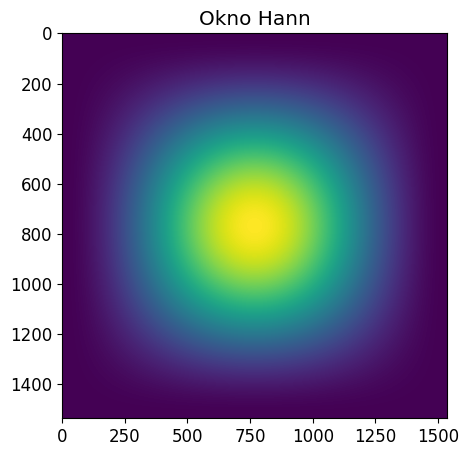
\includegraphics[width=5cm]{slika15.png}
\caption{Okenska funkcija uporabljena pri Fourierovi transformaciji.}
\end{figure}

V naslednjih podpoglavjih so prikazani rezultati za različna konvolucijska jedra.

\subsection{Prvo konvolucijsko jedro}

Rezultati čisčenja slik s prvim konvolucijskim jedrom so prikazani na sliki 16. Vidimo, da se usaj prva nezašumljena slika bolje vidi po dekonvoluciji. Prvzaprav so vse bolj ostre in imam problem le z vidljivostjo slik.

\begin{figure}[h!]
\centering
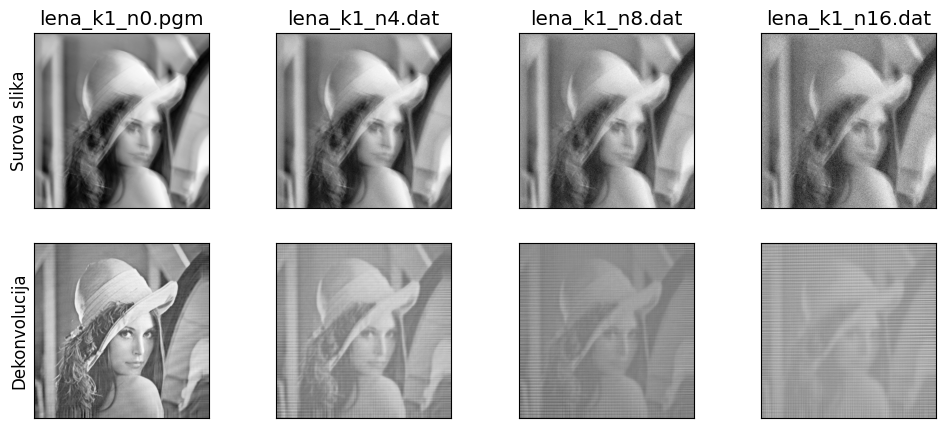
\includegraphics[width=12cm]{slika16.png}
\caption{Rezultati čisčenja slik s prvim konvolucijskim jedrom.}
\end{figure}

\subsection{Drugo konvolucijsko jedro}

Rezultati čiščenja slik z drugim konvolucijskim jedrom so prikazani na sliki 17. Tukaj sem imel največ težav in čiščenje slik ni bilo uspešno

\begin{figure}[h!]
\centering
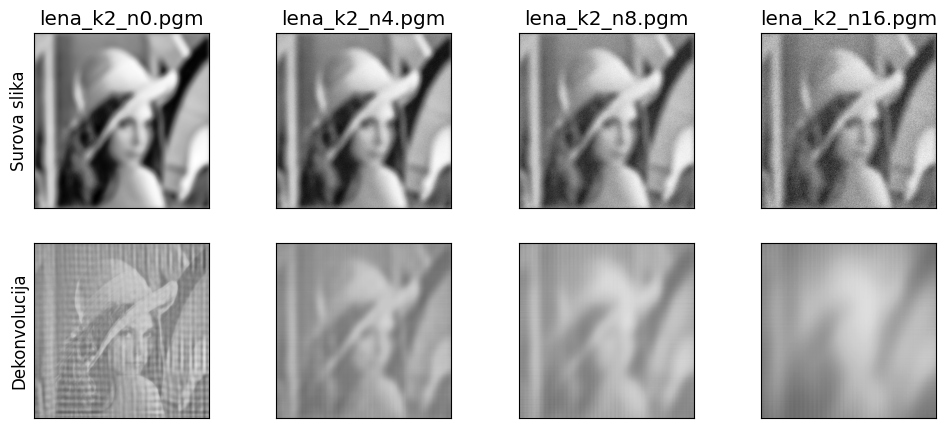
\includegraphics[width=12cm]{slika17.png}
\caption{Rezultati čisčenja slik z drugim konvolucijskim jedrom.}
\end{figure}

\subsection{Tretje konvolucijsko jedro}

Rezultati čiščenja slik s tretjim konvolucijskim jedrom so prikazani na sliki 18. Tukaj lahko vidimo, da so slike po čiščenju načeloma boljše kot pred njim.

\newpage

\begin{figure}[h!]
\centering
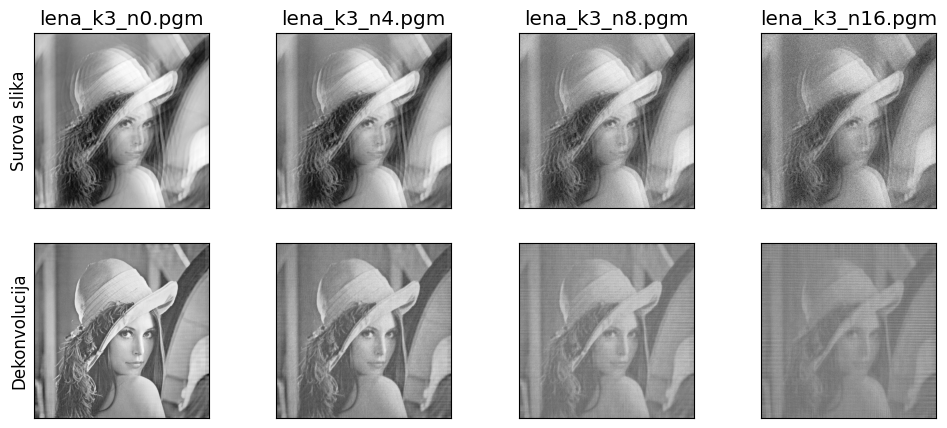
\includegraphics[width=12cm]{slika18.png}
\caption{Rezultati čisčenja slik z drugim konvolucijskim jedrom.}
\end{figure}

\section{Zaključek}

V nalogi smo se naučili postopke spektralne analize ter uporabe oken. Prav tako smo se naučili uporabljati Wienerjev filter, ki nam pomaga izločiti nezaželen šum iz signalov v frekvenčnem prostoru.

\end{document}